
%% x2-perception TDP, based on HumanoidLocoManipualtionChallenge_TDP.tex
%% V0.1
%% 2026/10/01
%% by Ben Beiter
%%
%% Based on RoboCupRescue_TDP.tex by Soeren Schwertfeger
%%
%% (requires IEEEtran.cls version 1.8b or later) with an IEEE
%% journal paper.
%%


%%*************************************************************************
%% Legal Notice:
%% This code is offered as-is without any warranty either expressed or
%% implied; without even the implied warranty of MERCHANTABILITY or
%% FITNESS FOR A PARTICULAR PURPOSE! 
%% User assumes all risk.
%% In no event shall the IEEE or any contributor to this code be liable for
%% any damages or losses, including, but not limited to, incidental,
%% consequential, or any other damages, resulting from the use or misuse
%% of any information contained here.
%%
%% All comments are the opinions of their respective authors and are not
%% necessarily endorsed by the IEEE.
%%
%% This work is distributed under the LaTeX Project Public License (LPPL)
%% ( http://www.latex-project.org/ ) version 1.3, and may be freely used,
%% distributed and modified. A copy of the LPPL, version 1.3, is included
%% in the base LaTeX documentation of all distributions of LaTeX released
%% 2003/12/01 or later.
%% Retain all contribution notices and credits.
%% ** Modified files should be clearly indicated as such, including  **
%% ** renaming them and changing author support contact information. **
%%*************************************************************************


% *** Authors should verify (and, if needed, correct) their LaTeX system  ***
% *** with the testflow diagnostic prior to trusting their LaTeX platform ***
% *** with production work. The IEEE's font choices and paper sizes can   ***
% *** trigger bugs that do not appear when using other class files.       ***                          ***
% The testflow support page is at:
% http://www.michaelshell.org/tex/testflow/



\documentclass[journal]{IEEEtran}
%
% If IEEEtran.cls has not been installed into the LaTeX system files,
% manually specify the path to it like:
% \documentclass[journal]{../sty/IEEEtran}


% Some very useful LaTeX packages include:
% (uncomment the ones you want to load)


% *** MISC UTILITY PACKAGES ***
%
%\usepackage{ifpdf}
% Heiko Oberdiek's ifpdf.sty is very useful if you need conditional
% compilation based on whether the output is pdf or dvi.
% usage:
% \ifpdf
%   % pdf code
% \else
%   % dvi code
% \fi
% The latest version of ifpdf.sty can be obtained from:
% http://www.ctan.org/pkg/ifpdf
% Also, note that IEEEtran.cls V1.7 and later provides a builtin
% \ifCLASSINFOpdf conditional that works the same way.
% When switching from latex to pdflatex and vice-versa, the compiler may
% have to be run twice to clear warning/error messages.

% *** CITATION PACKAGES ***
%
%\usepackage{cite}
% cite.sty was written by Donald Arseneau
% V1.6 and later of IEEEtran pre-defines the format of the cite.sty package
% \cite{} output to follow that of the IEEE. Loading the cite package will
% result in citation numbers being automatically sorted and properly
% "compressed/ranged". e.g., [1], [9], [2], [7], [5], [6] without using
% cite.sty will become [1], [2], [5]--[7], [9] using cite.sty. cite.sty's
% \cite will automatically add leading space, if needed. Use cite.sty's
% noadjust option (cite.sty V3.8 and later) if you want to turn this off
% such as if a citation ever needs to be enclosed in parenthesis.
% cite.sty is already installed on most LaTeX systems. Be sure and use
% version 5.0 (2009-03-20) and later if using hyperref.sty.
% The latest version can be obtained at:
% http://www.ctan.org/pkg/cite
% The documentation is contained in the cite.sty file itself.

\usepackage[pdfborder=0 0 0,colorlinks=true,urlcolor=blue,citecolor=blue, linkcolor=blue]{hyperref}

% *** GRAPHICS RELATED PACKAGES ***
%
\ifCLASSINFOpdf
  \usepackage[pdftex]{graphicx}
  % declare the path(s) where your graphic files are
  % \graphicspath{{../pdf/}{../jpeg/}}
  % and their extensions so you won't have to specify these with
  % every instance of \includegraphics
  % \DeclareGraphicsExtensions{.pdf,.jpeg,.png}
\else
  % or other class option (dvipsone, dvipdf, if not using dvips). graphicx
  % will default to the driver specified in the system graphics.cfg if no
  % driver is specified.
  % \usepackage[dvips]{graphicx}
  % declare the path(s) where your graphic files are
  % \graphicspath{{../eps/}}
  % and their extensions so you won't have to specify these with
  % every instance of \includegraphics
  % \DeclareGraphicsExtensions{.eps}
\fi
% graphicx was written by David Carlisle and Sebastian Rahtz. It is
% required if you want graphics, photos, etc. graphicx.sty is already
% installed on most LaTeX systems. The latest version and documentation
% can be obtained at: 
% http://www.ctan.org/pkg/graphicx
% Another good source of documentation is "Using Imported Graphics in
% LaTeX2e" by Keith Reckdahl which can be found at:
% http://www.ctan.org/pkg/epslatex
%
% latex, and pdflatex in dvi mode, support graphics in encapsulated
% postscript (.eps) format. pdflatex in pdf mode supports graphics
% in .pdf, .jpeg, .png and .mps (metapost) formats. Users should ensure
% that all non-photo figures use a vector format (.eps, .pdf, .mps) and
% not a bitmapped formats (.jpeg, .png). The IEEE frowns on bitmapped formats
% which can result in "jaggedy"/blurry rendering of lines and letters as
% well as large increases in file sizes.
%
% You can find documentation about the pdfTeX application at:
% http://www.tug.org/applications/pdftex

% *** MATH PACKAGES ***
%
%\usepackage{amsmath}
% A popular package from the American Mathematical Society that provides
% many useful and powerful commands for dealing with mathematics.
%
% Note that the amsmath package sets \interdisplaylinepenalty to 10000
% thus preventing page breaks from occurring within multiline equations. Use:
%\interdisplaylinepenalty=2500
% after loading amsmath to restore such page breaks as IEEEtran.cls normally
% does. amsmath.sty is already installed on most LaTeX systems. The latest
% version and documentation can be obtained at:
% http://www.ctan.org/pkg/amsmath

% *** SPECIALIZED LIST PACKAGES ***
%
%\usepackage{algorithmic}
% algorithmic.sty was written by Peter Williams and Rogerio Brito.
% This package provides an algorithmic environment fo describing algorithms.
% You can use the algorithmic environment in-text or within a figure
% environment to provide for a floating algorithm. Do NOT use the algorithm
% floating environment provided by algorithm.sty (by the same authors) or
% algorithm2e.sty (by Christophe Fiorio) as the IEEE does not use dedicated
% algorithm float types and packages that provide these will not provide
% correct IEEE style captions. The latest version and documentation of
% algorithmic.sty can be obtained at:
% http://www.ctan.org/pkg/algorithms
% Also of interest may be the (relatively newer and more customizable)
% algorithmicx.sty package by Szasz Janos:
% http://www.ctan.org/pkg/algorithmicx

% *** ALIGNMENT PACKAGES ***
%
%\usepackage{array}
% Frank Mittelbach's and David Carlisle's array.sty patches and improves
% the standard LaTeX2e array and tabular environments to provide better
% appearance and additional user controls. As the default LaTeX2e table
% generation code is lacking to the point of almost being broken with
% respect to the quality of the end results, all users are strongly
% advised to use an enhanced (at the very least that provided by array.sty)
% set of table tools. array.sty is already installed on most systems. The
% latest version and documentation can be obtained at:
% http://www.ctan.org/pkg/array


% IEEEtran contains the IEEEeqnarray family of commands that can be used to
% generate multiline equations as well as matrices, tables, etc., of high
% quality.

% *** SUBFIGURE PACKAGES ***
%\ifCLASSOPTIONcompsoc
%  \usepackage[caption=false,font=normalsize,labelfont=sf,textfont=sf]{subfig}
%\else
%  \usepackage[caption=false,font=footnotesize]{subfig}
%\fi
% subfig.sty, written by Steven Douglas Cochran, is the modern replacement
% for subfigure.sty, the latter of which is no longer maintained and is
% incompatible with some LaTeX packages including fixltx2e. However,
% subfig.sty requires and automatically loads Axel Sommerfeldt's caption.sty
% which will override IEEEtran.cls' handling of captions and this will result
% in non-IEEE style figure/table captions. To prevent this problem, be sure
% and invoke subfig.sty's "caption=false" package option (available since
% subfig.sty version 1.3, 2005/06/28) as this is will preserve IEEEtran.cls
% handling of captions.
% Note that the Computer Society format requires a larger sans serif font
% than the serif footnote size font used in traditional IEEE formatting
% and thus the need to invoke different subfig.sty package options depending
% on whether compsoc mode has been enabled.
%
% The latest version and documentation of subfig.sty can be obtained at:
% http://www.ctan.org/pkg/subfig

% *** FLOAT PACKAGES ***
%
%\usepackage{fixltx2e}
% fixltx2e, the successor to the earlier fix2col.sty, was written by
% Frank Mittelbach and David Carlisle. This package corrects a few problems
% in the LaTeX2e kernel, the most notable of which is that in current
% LaTeX2e releases, the ordering of single and double column floats is not
% guaranteed to be preserved. Thus, an unpatched LaTeX2e can allow a
% single column figure to be placed prior to an earlier double column
% figure.
% Be aware that LaTeX2e kernels dated 2015 and later have fixltx2e.sty's
% corrections already built into the system in which case a warning will
% be issued if an attempt is made to load fixltx2e.sty as it is no longer
% needed.
% The latest version and documentation can be found at:
% http://www.ctan.org/pkg/fixltx2e


%\usepackage{stfloats}
% stfloats.sty was written by Sigitas Tolusis. This package gives LaTeX2e
% the ability to do double column floats at the bottom of the page as well
% as the top. (e.g., "\begin{figure*}[!b]" is not normally possible in
% LaTeX2e). It also provides a command:
%\fnbelowfloat
% to enable the placement of footnotes below bottom floats (the standard
% LaTeX2e kernel puts them above bottom floats). This is an invasive package
% which rewrites many portions of the LaTeX2e float routines. It may not work
% with other packages that modify the LaTeX2e float routines. The latest
% version and documentation can be obtained at:
% http://www.ctan.org/pkg/stfloats
% Do not use the stfloats baselinefloat ability as the IEEE does not allow
% \baselineskip to stretch. Authors submitting work to the IEEE should note
% that the IEEE rarely uses double column equations and that authors should try
% to avoid such use. Do not be tempted to use the cuted.sty or midfloat.sty
% packages (also by Sigitas Tolusis) as the IEEE does not format its papers in
% such ways.
% Do not attempt to use stfloats with fixltx2e as they are incompatible.
% Instead, use Morten Hogholm'a dblfloatfix which combines the features
% of both fixltx2e and stfloats:
%
% \usepackage{dblfloatfix}
% The latest version can be found at:
% http://www.ctan.org/pkg/dblfloatfix


%\ifCLASSOPTIONcaptionsoff
%  \usepackage[nomarkers]{endfloat}
% \let\MYoriglatexcaption\caption
% \renewcommand{\caption}[2][\relax]{\MYoriglatexcaption[#2]{#2}}
%\fi
% endfloat.sty was written by James Darrell McCauley, Jeff Goldberg and 
% Axel Sommerfeldt. This package may be useful when used in conjunction with 
% IEEEtran.cls'  captionsoff option. Some IEEE journals/societies require that
% submissions have lists of figures/tables at the end of the paper and that
% figures/tables without any captions are placed on a page by themselves at
% the end of the document. If needed, the draftcls IEEEtran class option or
% \CLASSINPUTbaselinestretch interface can be used to increase the line
% spacing as well. Be sure and use the nomarkers option of endfloat to
% prevent endfloat from "marking" where the figures would have been placed
% in the text. The two hack lines of code above are a slight modification of
% that suggested by in the endfloat docs (section 8.4.1) to ensure that
% the full captions always appear in the list of figures/tables - even if
% the user used the short optional argument of \caption[]{}.
% IEEE papers do not typically make use of \caption[]'s optional argument,
% so this should not be an issue. A similar trick can be used to disable
% captions of packages such as subfig.sty that lack options to turn off
% the subcaptions:
% For subfig.sty:
% \let\MYorigsubfloat\subfloat
% \renewcommand{\subfloat}[2][\relax]{\MYorigsubfloat[]{#2}}
% However, the above trick will not work if both optional arguments of
% the \subfloat command are used. Furthermore, there needs to be a
% description of each subfigure *somewhere* and endfloat does not add
% subfigure captions to its list of figures. Thus, the best approach is to
% avoid the use of subfigure captions (many IEEE journals avoid them anyway)
% and instead reference/explain all the subfigures within the main caption.
% The latest version of endfloat.sty and its documentation can obtained at:
% http://www.ctan.org/pkg/endfloat
%
% The IEEEtran \ifCLASSOPTIONcaptionsoff conditional can also be used
% later in the document, say, to conditionally put the References on a 
% page by themselves.


% *** PDF, URL AND HYPERLINK PACKAGES ***
%
\usepackage{url}
% url.sty was written by Donald Arseneau. It provides better support for
% handling and breaking URLs. url.sty is already installed on most LaTeX
% systems. The latest version and documentation can be obtained at:
% http://www.ctan.org/pkg/url
% Basically, \url{my_url_here}.


% *** Do not adjust lengths that control margins, column widths, etc. ***
% *** Do not use packages that alter fonts (such as pslatex).         ***
% There should be no need to do such things with IEEEtran.cls V1.6 and later.
% (Unless specifically asked to do so by the journal or conference you plan
% to submit to, of course. )

\begin{document}

\title{Humanoid Loco-Manipulation Challenge 2026 Team Description Paper \\
 x2-perception}

\author{Sitarama~Chekuri}

\markboth{Loco-Manipulation Challenge TDP}%
{x2-perception}

\maketitle

\begin{flushleft}
\textbf{Info}\\
\hspace{10pt} Team Name: \hfill x2-perception\\
\hspace{10pt} Team Institution: \hfill Independent\\
\hspace{10pt} Team Country: \hfill USA\\
\hspace{10pt} Team Leader: \hfill Sitarama Chekuri\\
\hspace{10pt} Team URL: \hfill \url{https://x2-perception.github.io}
\\
\vspace{5pt}
\hspace{10pt} RoboCup TDP collection: 
 \url{https://tdp.robocup.org/tdp/}
\end{flushleft}

\begin{abstract}
We will compete in the mobility tasks with the AgiBot X2 provided at the conference, running our own perceptive locomotion
software. Its core is Adaptive Contact Planning (ACP), a learned perceptive locomotion controller. ACP was originally developed on the Unitree G1, with height maps from a
LiDAR; we implemented it for the AgiBot X2 and replaced the LiDAR with a custom-mounted depth camera. The X2's built-in depth
camera cannot see the ground close to its feet, so we add an Intel RealSense depth camera on a 3D-printed chest mount and train a small depth student
that turns the camera image into the height maps ACP expects, using only proprioception and the depth stream. In a held-out MuJoCo replica of the competition
apparatus, ACP on the depth camera alone completes the full mobility route in 92\% of trials (46 of 50, with realistic
depth-camera noise in the loop); with simulator height maps instead of the camera, ACP completes it in 99\% of 200 trials. On the
real X2 the same policy runs zero-shot on the robot's onboard computer, with no training on the real robot: it stands steadily,
recovers from pushes, and walks an outdoor course of patio, gravel, a step down and a doorway under gamepad control. Project page:
\url{https://x2-perception.github.io}.
\end{abstract}

\begin{IEEEkeywords}
Loco-Manipulation Challenge, Team Description Paper, humanoid locomotion, depth perception, reinforcement learning.
\end{IEEEkeywords}

\IEEEpeerreviewmaketitle

\section{Introduction}
\IEEEPARstart{O}{ur} team focuses on the mobility part of the challenge: stepping over obstacles, crossing ramps, walking on
flat ground and climbing stairs, with the robot choosing every foothold from what it sees. We use the AgiBot X2 provided
by Ultimate Bots and bring software and a chest camera mount.

Learned perceptive locomotion builds on teacher-student training in simulation~\cite{lee2020,miki2022} and has been shown
from depth cameras on quadrupeds~\cite{robotparkour,extremeparkour,anymalparkour} and humanoids~\cite{humanoidparkour,
deepparkour,php,nowyousee,rpl,echo,cref,dpl,gaitunder}, and from LiDAR elevation maps~\cite{pim,beamdojo,gallant,omnistairs,
guidewalk,polygmap}. Our approach is learned and simulation-first. We ported three published perceptive-locomotion methods to the X2: ACP~\cite{acp}, Hiking in the Wild~\cite{hiking} (depth camera) and SSR~\cite{ssr} (depth camera
with memory). All three are scored by one evaluation that never trains on the competition apparatus: a MuJoCo model of the
apparatus built from its CAD, with randomised physics. ACP is the strongest (99\% of full-route trials with simulator height maps), so it is our
competition system. ACP was originally developed on the Unitree G1 with LiDAR height maps; we re-implemented it for the
X2, trained it from scratch, and replaced the LiDAR with a depth camera on a
custom chest mount: a depth student we built supplies the height maps from that camera.

At the competition the operator steers with a gamepad (walk, turn, stop) while the robot plans its own footholds from the
depth camera. The success rates in Table~\ref{tab:results} come from simulation; on the real X2 the same policy now stands,
walks and turns zero-shot (Section~\ref{sec:realrobot}).

\begin{figure}[!t]
\centering
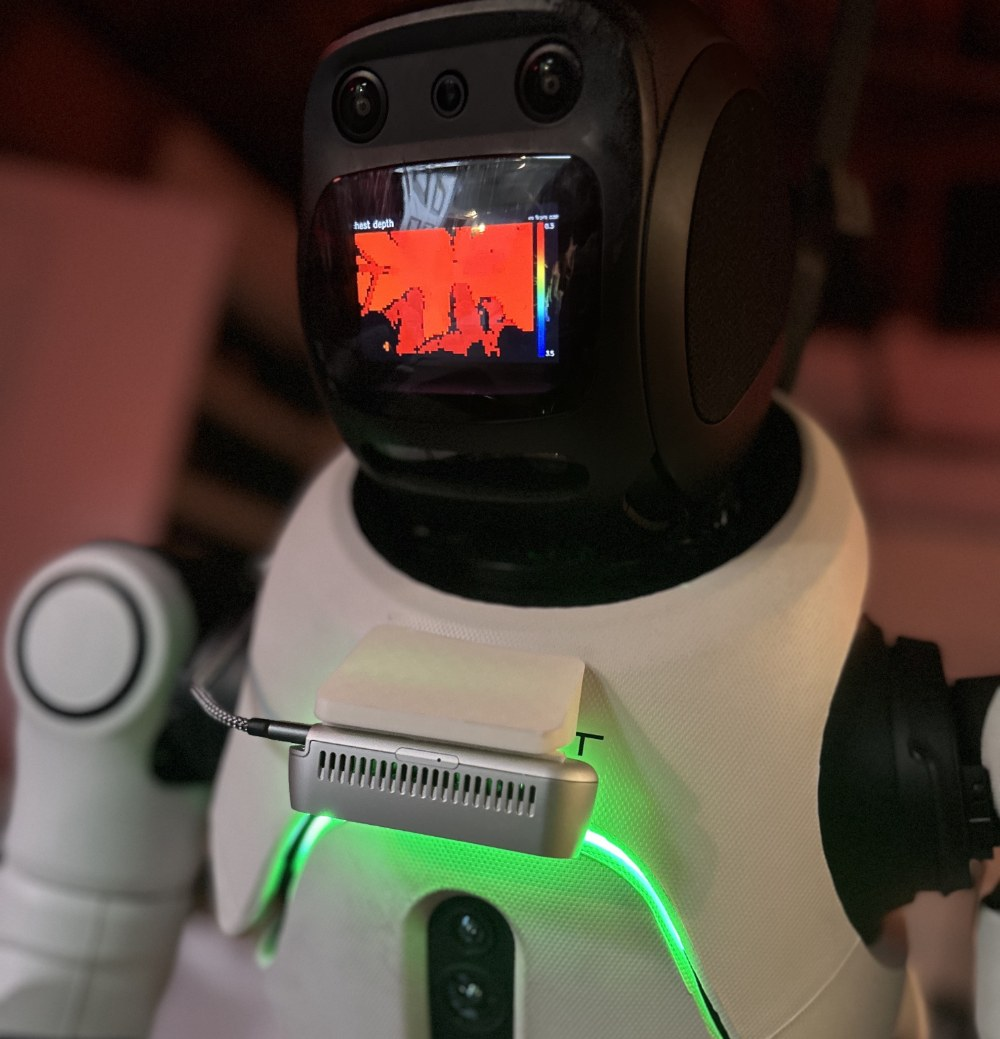
\includegraphics[width=\linewidth]{figs/robot_photo}
\caption{The AgiBot X2 with our chest-mounted Intel RealSense depth camera. The face display shows the live chest depth image
while our perception stack runs.}
\label{fig:robotPhoto}
\end{figure}

\section{System Description}

\subsection{Hardware and Design}
We will use the AgiBot X2 provided at the conference, with a custom-mounted Intel RealSense depth camera on its chest
(Fig.~\ref{fig:perception}) that connects to the robot's onboard computer (PC2) over USB.

\begin{figure*}[!t]
\centering
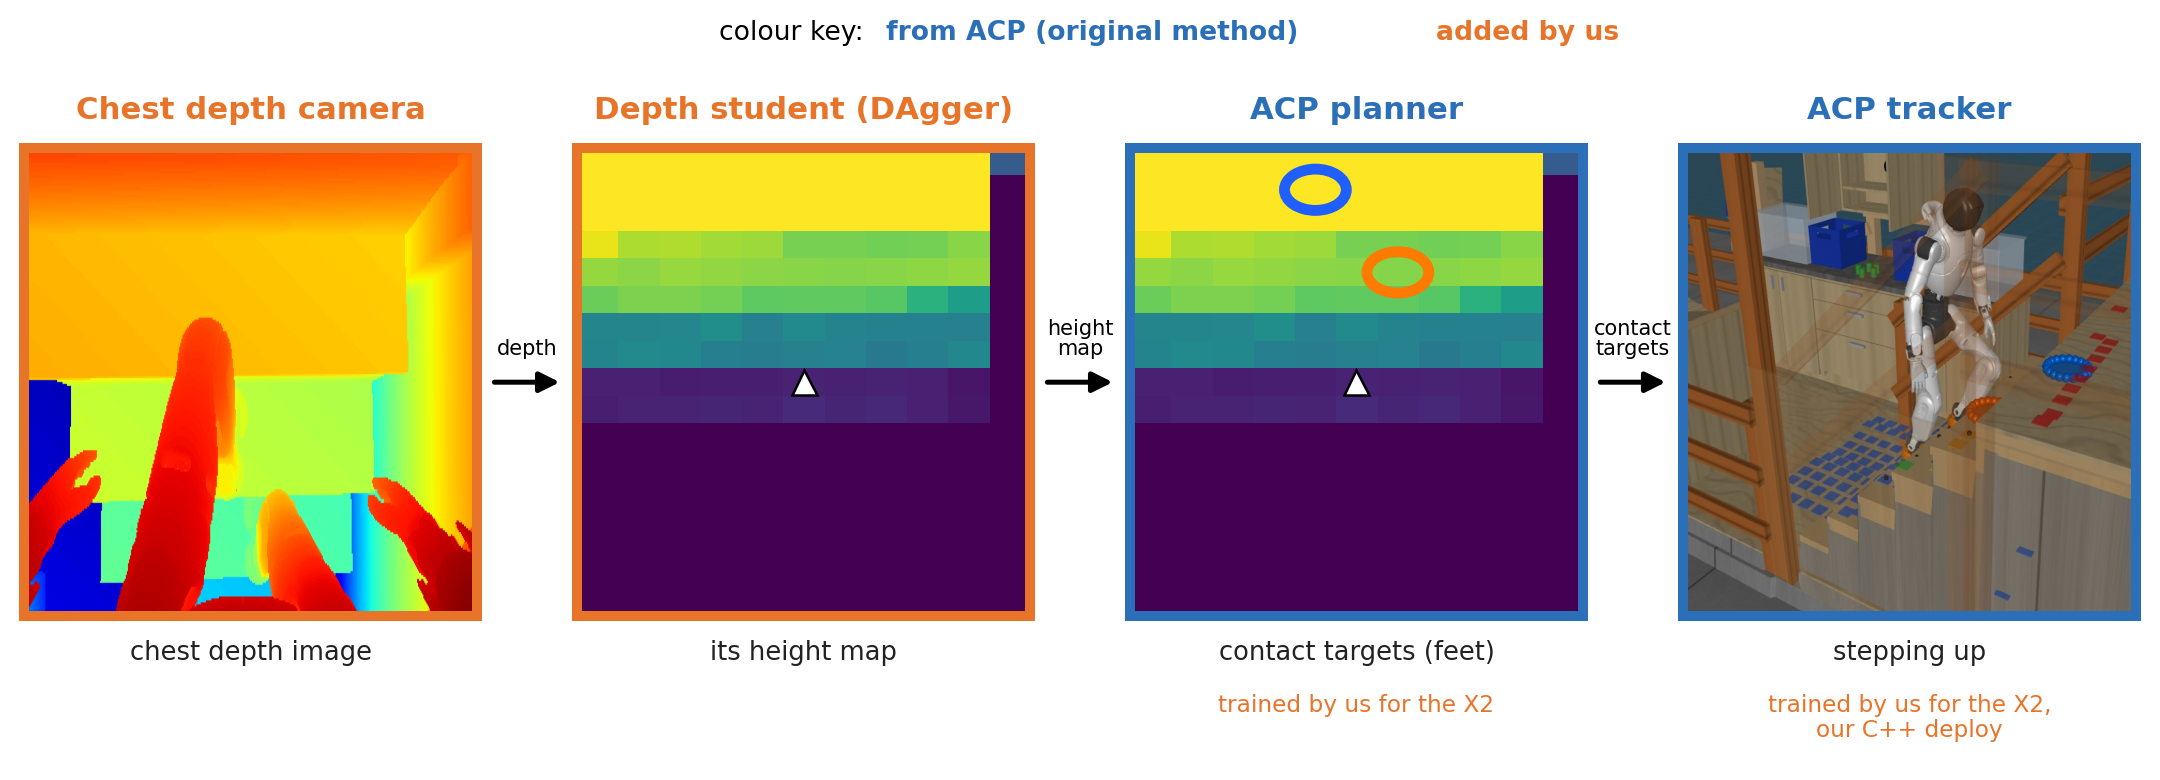
\includegraphics[width=\textwidth]{figs/pipeline}
\caption{Our perception-to-motion pipeline at one moment of a simulated stair climb on the apparatus. The chest depth camera
and the depth student (trained with DAgger) are ours; the planner and tracker are ACP~\cite{acp}, which we re-implemented and
trained for the X2 and deploy with our own robot software. Left to right: the chest depth image (the steps ahead and the robot's
own hands and legs), the student's height map from it (forward up; the steps rise ahead), the planner's foot targets on that
map (rings: left foot blue, right foot orange), and the tracker stepping up.}
\label{fig:pipeline}
\end{figure*}

\subsection{Sensing, SLAM, and State Estimation}
The robot senses the terrain with the chest depth camera alone (Fig.~\ref{fig:pipeline}), where the original ACP on the Unitree G1 used a LiDAR; the
policy also uses the robot's proprioception (IMU and joint states). A learned depth student turns the depth stream, together
with the camera pose from the robot's kinematics, into the local height maps ACP expects, and keeps a short memory so the
ground under the feet stays known after it leaves the camera's view. It is trained in simulation against the true terrain with DAgger~\cite{dagger},
with depth-camera noise modelled. We do not use SLAM: the height map is local and centred on the robot.

\subsection{Motion Planning and Whole-Body Control}
Motion planning and whole-body control are ACP~\cite{acp}, re-implemented for the X2 and trained from scratch with
PPO~\cite{ppo} in simulation on our terrain set, with the height maps supplied by our depth student instead of a LiDAR. Hiking in the
Wild and SSR are kept as alternatives (Table~\ref{tab:results}).

\subsection{Autonomy and Behavior Generation}
Foothold selection, balance and stepping are autonomous: the operator gives the walking direction and turns, and the policy
decides where and how to step, including over obstacles and on stairs. In our evaluation the same policy also follows a
route through the whole apparatus from waypoint goals.

\subsection{User Interface}
The operator drives the robot with a gamepad: walk, turn, stop, stand, and an emergency stop, with a deadman control so the
robot stops when the operator lets go. A status display shows the controller state, and the robot drops to a safe state if
it tilts too far or its sensor or command data stop arriving.

\subsection{Communication}
The policy runs on the robot, so operation needs no network link. The operator's gamepad connects to the robot over
Bluetooth; if its connection drops, the robot stops and stands.

\section{Competition Strategy}
We will attempt the Mobility part with all four tasks: Stepover Obstacles, Crossing Ramps, Flat Ground Walking, and Stairs
Ascend and Descend. These are what our system is built and tested for; Table~\ref{tab:results} reports its success on our
replica of the full mobility route. We do not plan to attempt the manipulation or loco-manipulation parts this year.

\begin{figure}[!t]
\centering
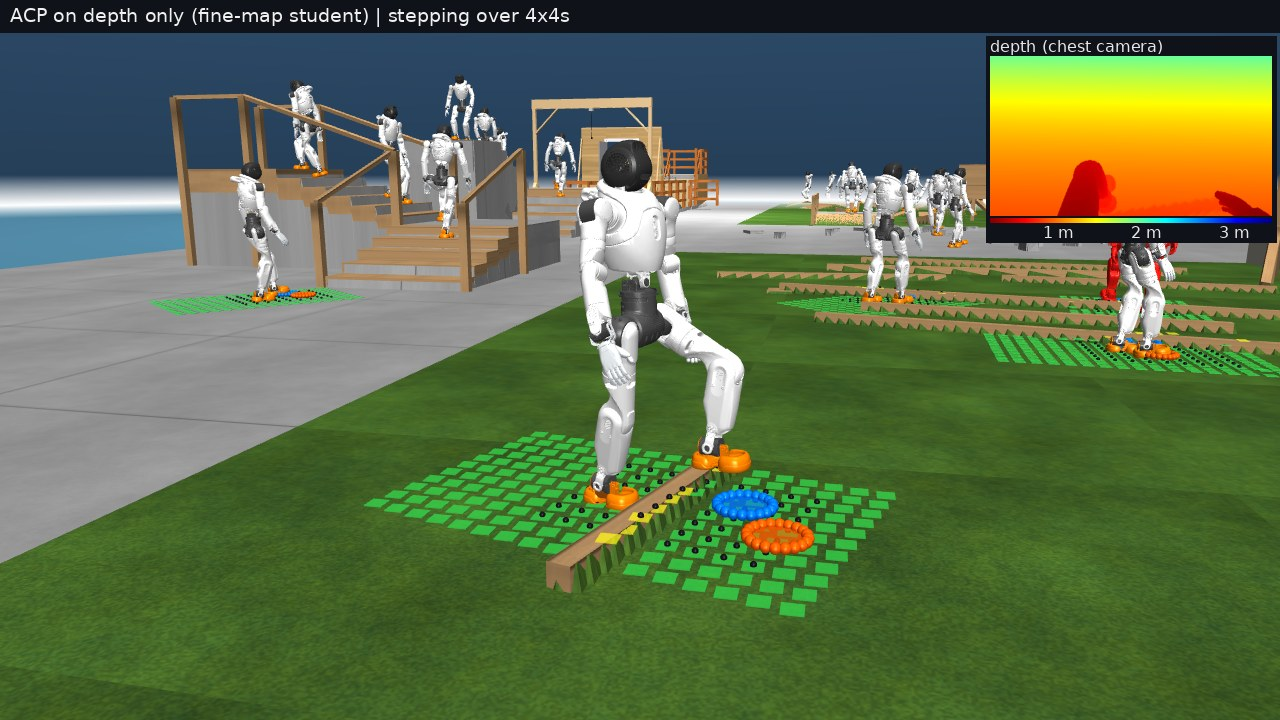
\includegraphics[width=\linewidth]{figs/perception_4x4}
\caption{Stepping over a 4x4 in simulation, driven by depth only. Tiles: the planner height map from the depth student
(green level, yellow 4x4 height); dots: tracker map; rings: planned footholds. Inset: the chest depth image.}
\label{fig:perception}
\end{figure}

\section{Experiments}
\label{sec:experiments}

\subsection{Held-out apparatus evaluation}
Every policy is scored by the same MuJoCo evaluation: a model of the competition apparatus built from its CAD (door, two
4x4 stepovers, crossing ramps, a wall, stairs to a landing, buttons), traversed as one full route, plus a second, unseen
apparatus (NIST). Neither is used in training. Each trial uses domain randomization and pushes;
a trial succeeds when the robot completes the route without falling.

\begin{table}[!t]
\renewcommand{\arraystretch}{1.1}
\caption{Full-route success in the held-out MuJoCo apparatus evaluation}
\label{tab:results}
\centering
\tabcolsep=0.08cm
\begin{tabular}{|l|l|c|c|}
\hline
Policy & Terrain input & Our replica & NIST \\
\hline
ACP & simulator maps & 198/200 & 155/200 \\
ACP + depth student & chest depth only & 46/50 & -- \\
Hiking in the Wild & chest depth & not yet evaluated & -- \\
SSR & chest depth & not yet evaluated & -- \\
\hline
\end{tabular}
\end{table}

\subsection{Depth student}
With realistic depth-camera noise in the loop, ACP on the depth student completes the route in 46 of 50 trials (92\%),
against 99\% for ACP with simulator height maps (Table~\ref{tab:results}). Across our terrain park (4x4s, blocks, ramps,
wedges, straight, L- and U-shaped stairs, furnished rooms and corridors), 61 of 63 episodes succeed
(Fig.~\ref{fig:apparatus}).

\subsection{Real robot}
\label{sec:realrobot}
The robot-side software uses only what the robot has (IMU, joints, depth camera, gamepad), reproduces the evaluation's
controller exactly, and runs entirely on the X2's onboard computer. We first test every change in a simulation of the X2's
own software interface, then on the real robot; a flight recorder logs each control step so a real-robot run can be replayed
and compared with simulation. This found the main deployment issue: a mismatch between where our code assumed the robot's IMU
sits and where it actually is, which we reproduced in simulation and fixed. With that fixed, the policy trained only in
simulation runs zero-shot on the real X2. Standing still, its torso stays within about 3\textdegree{} of upright; when pushed it
recovers from tilts of up to about 10\textdegree{}, comparable to the GR00T whole-body controller (SONIC)
on the same robot. Under gamepad control it walked an outdoor course around a house: a patio, a step down onto gravel, gravel next to a
path, and through a doorway (Fig.~\ref{fig:realwalk}). In first trials it also stepped over a 4x4 lying across its path, but
usually only after first touching it: small obstacles close to the feet are not yet kept reliably in the depth student's map
on the real camera, which is our current work.

\begin{figure}[!t]
\centering
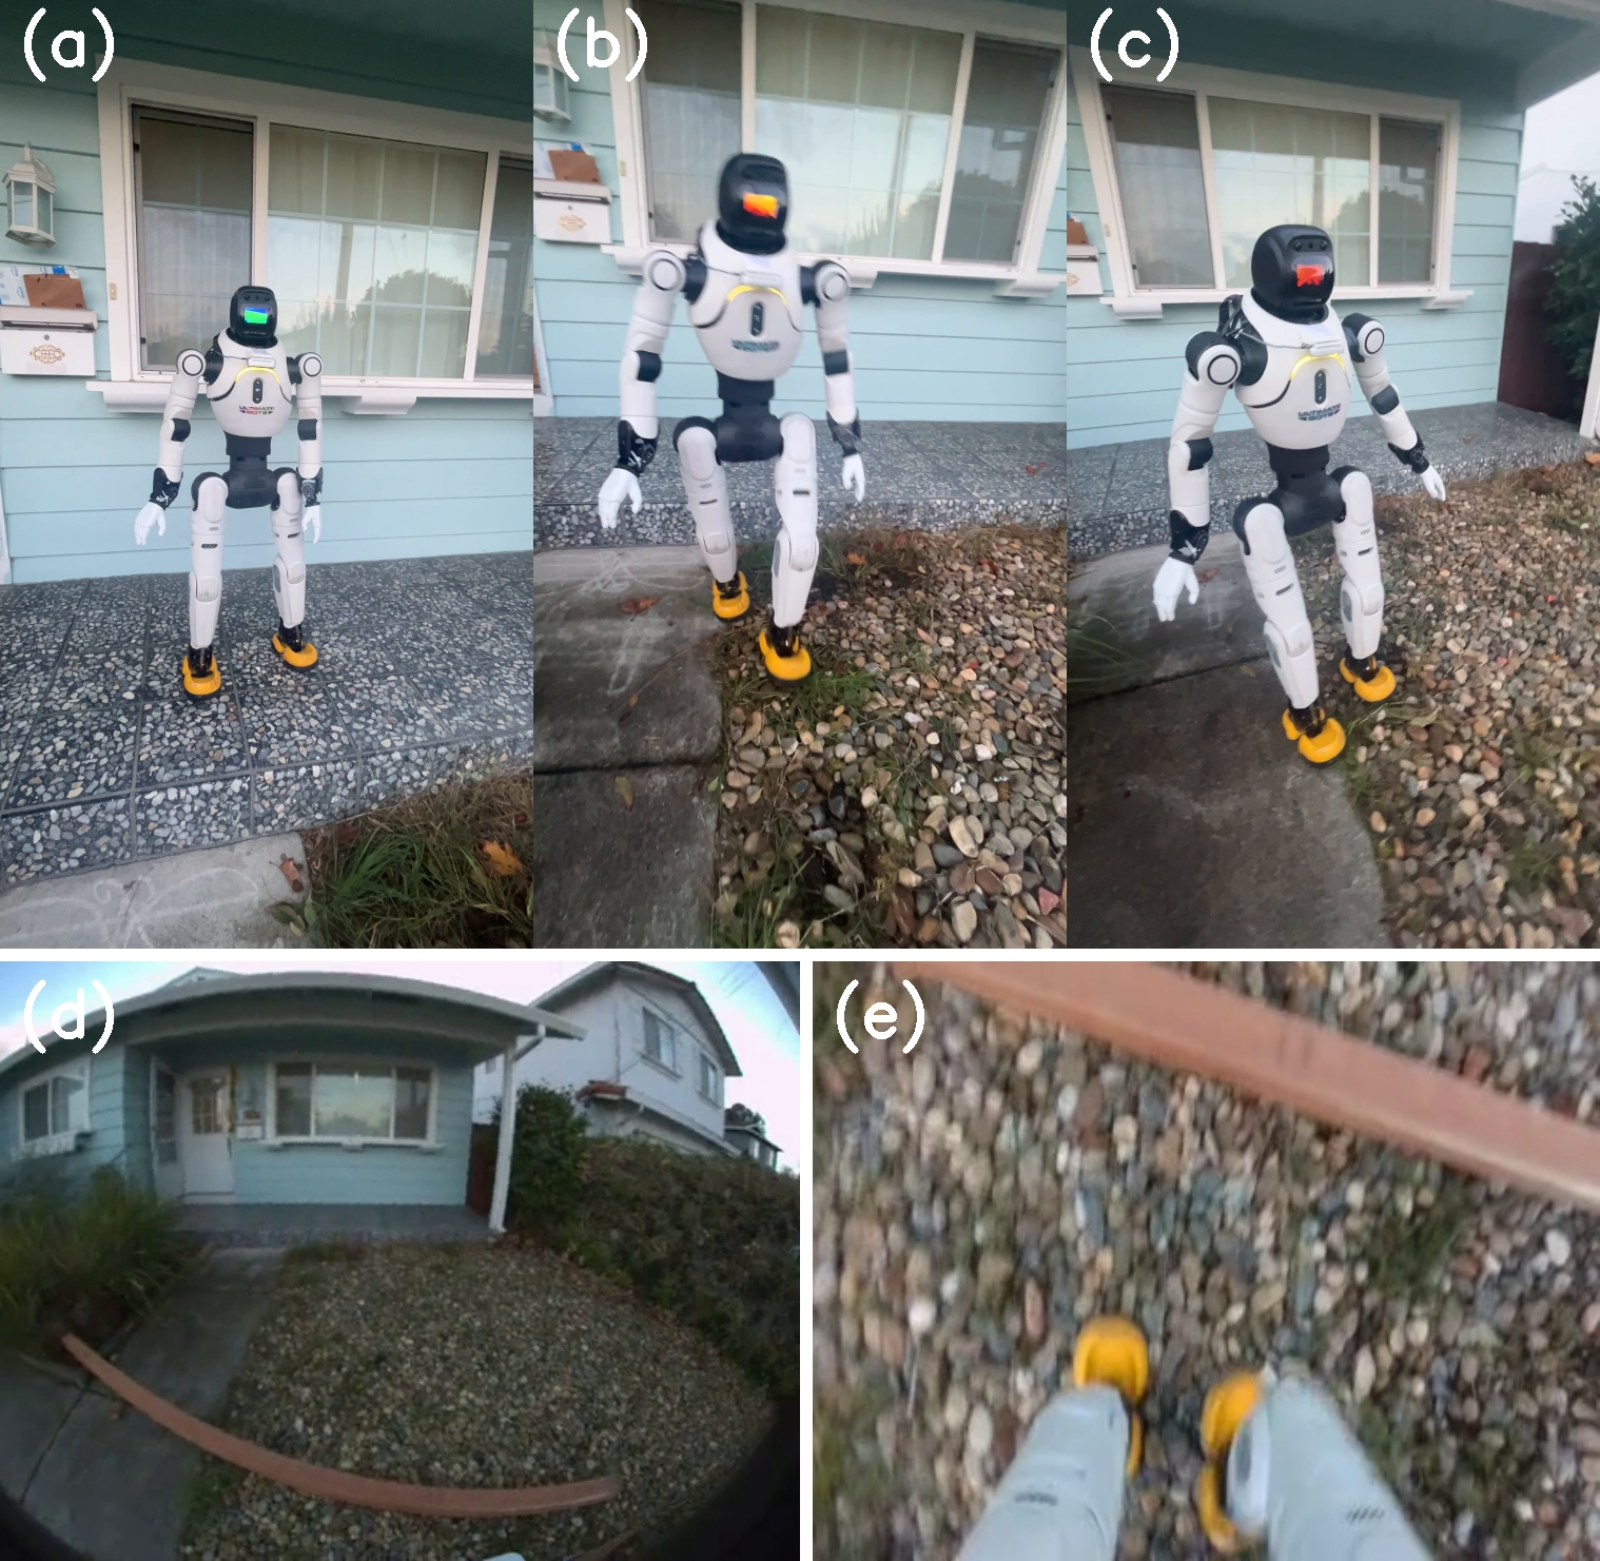
\includegraphics[width=\linewidth]{figs/real_walk}
\caption{The real X2 running ACP with the depth student on its chest camera, zero-shot. (a)--(c) Walking off a patio and down
onto gravel. (d), (e) The robot's own head and chest camera views on the outdoor course, with a 4x4 lying on the gravel.}
\label{fig:realwalk}
\end{figure}

\begin{figure}[!t]
\centering
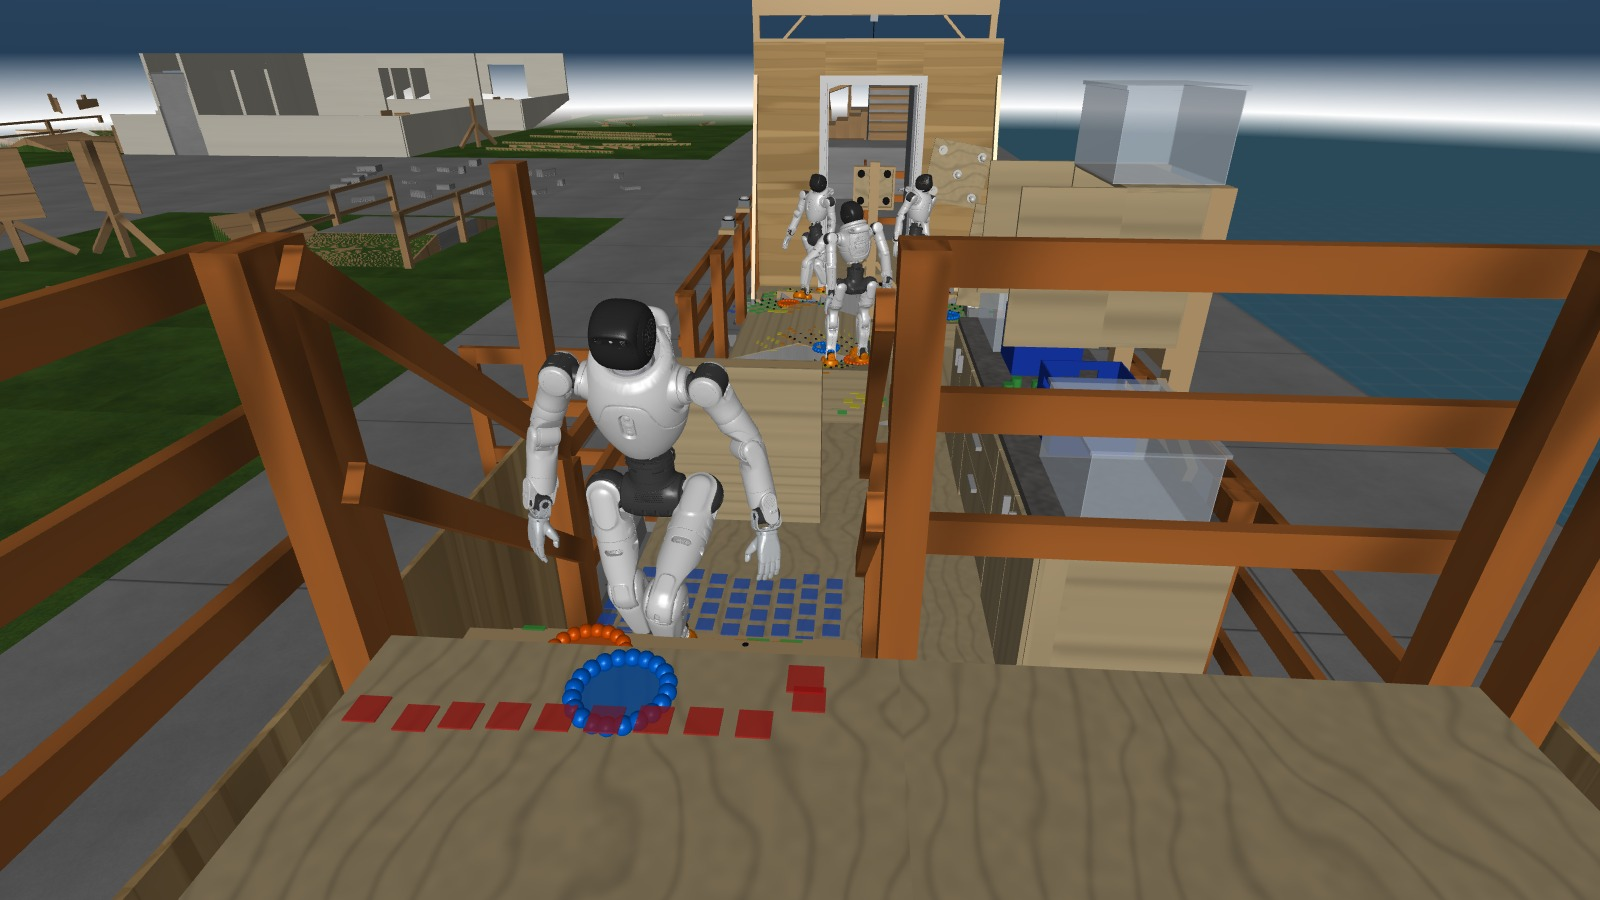
\includegraphics[width=\linewidth]{figs/apparatus}
\caption{ACP on depth only on our apparatus replica, seen from the stairs: one evaluation run shown at four moments, stepping
over the two 4x4s (top), crossing the ramps (middle) and climbing the stairs (bottom). Tiles: the height map from the depth
student (green level, yellow 4x4 height, orange a stair step, red higher, blue below); rings: planned footholds.}
\label{fig:apparatus}
\end{figure}

\section{Conclusion}
Our team brings learned, perception-driven locomotion to the mobility tasks: ACP plans footholds from a chest depth camera
and completes 92\% of full routes in our held-out simulation on the camera alone (99\% with simulator height maps). On the
real X2 the same policy already stands, recovers from pushes and walks an outdoor course zero-shot. Next is reliable stepping
over obstacles before contact on the real camera, then the apparatus tasks one by one. All code, trained models and the
evaluation are public.

\appendices

\section{Team members and Their Contributions}
\begin{itemize}
\item Sitarama Chekuri: team lead; system design, training, evaluation, deployment and hardware (camera mount).
\end{itemize}
Much of the engineering was carried out with AI coding agents (Anthropic Claude) under the author's direction.

\section{Lists}
\subsection{Systems List}
\begin{table}[!h]
\renewcommand{\arraystretch}{1}
 \tabcolsep=0.1cm
\caption{Humanoid System}
\label{tab:SystemRobot1}
\centering
\begin{tabular}{|l|r|}
\hline
Attribute & Value \\ \hline
Name & AgiBot X2 (provided) \\
Locomotion & bipedal \\
Height & 1.31 m \\
System weight & about 39 kg* \\
Degrees of freedom & 31 \\
Onboard computer & NVIDIA Jetson Orin NX 16 GB \\
Added sensor & chest depth camera (USB) \\
Operator input & gamepad \\
\hline
\end{tabular}
\end{table}

\subsection{Software List}
\begin{table}[!h]
\renewcommand{\arraystretch}{1}
 \tabcolsep=0.1cm
\caption{Software List}
\label{tab:SoftwareList}
\centering
\begin{tabular}{|c|c|c|c|}
\hline
Name & Version & License & Usage \\
\hline
\href{https://github.com/google-deepmind/mujoco_warp}{MuJoCo Warp} & 3.17 & Apache 2.0 & ACP training (GPU) \\
\href{https://pytorch.org}{PyTorch} & 2.10 & BSD & policy, depth student \\
\href{https://isaac-sim.github.io/IsaacLab}{Isaac Lab} & -- & BSD & Hiking training \\
\href{https://mujoco.org}{MuJoCo} & 3.17 & Apache 2.0 & held-out evaluation \\
\href{https://github.com/meetsitaram/terrain-park}{terrain-park} & -- & open & terrain, apparatus \\
\href{https://docs.ros.org/en/humble/}{ROS 2} & Humble & Apache 2.0 & robot interface \\
\href{https://x2-aimdk.agibot.com}{AgiBot AimDK} & -- & vendor & X2 joints, IMU \\
\href{https://onnxruntime.ai}{ONNX Runtime} & 1.20 & MIT & onboard inference \\
\href{https://github.com/IntelRealSense/librealsense}{RealSense} & 2.56 & Apache 2.0 & depth camera \\
\href{https://github.com/NVlabs/GR00T-WholeBodyControl}{GR00T WBC} & -- & Apache 2.0 & sim-to-sim tests \\
\hline
\end{tabular}
\end{table}

\bibliographystyle{IEEEtran}
\bibliography{references}

\end{document}
